\section{Más}

\begin{frame}[fragile]{Hoogle}
  Hoogle permite buscar funciones por tipo entre las librerías
  estándar de Haskell:
  
  \begin{center}
  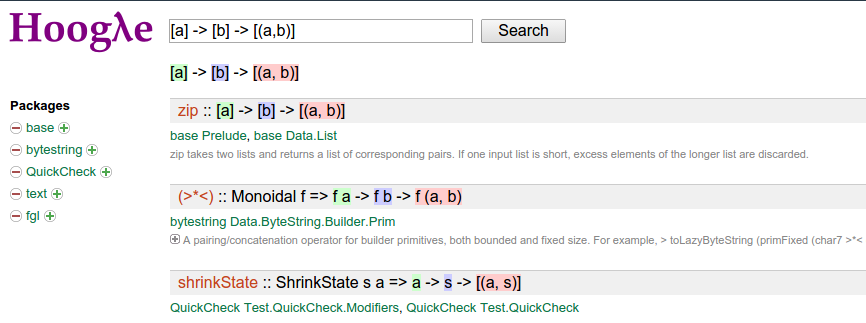
\includegraphics[scale=0.35]{./images/hoogle.png}
  \end{center}
\end{frame}


\begin{frame}[fragile]{Demostraciones}
  Como las funciones no tienen efectos secundarios, podemos razonar la
  corrección del código por inducción:

  \begin{lstlisting}[language=haskell]
qsort []     = []
qsort (x:xs) = qsort [y | y<-xs, y<=x]
            ++ [x]
            ++ qsort [y | y<-xs, y>x]
  \end{lstlisting}

  \textbf{Demostración:} \textit{Quicksort} funciona porque:
  \begin{itemize}
   \item ordena correctamente una lista vacía.
   \item la lista creada mantiene el orden entre las tres partes
  \end{itemize}
\end{frame}


\begin{frame}[fragile]{Idris}
  \textbf{Idris}, construido encima de Haskell, demuestra
  matemáticamente que los
  programas son correctos.
  
  \begin{center}
  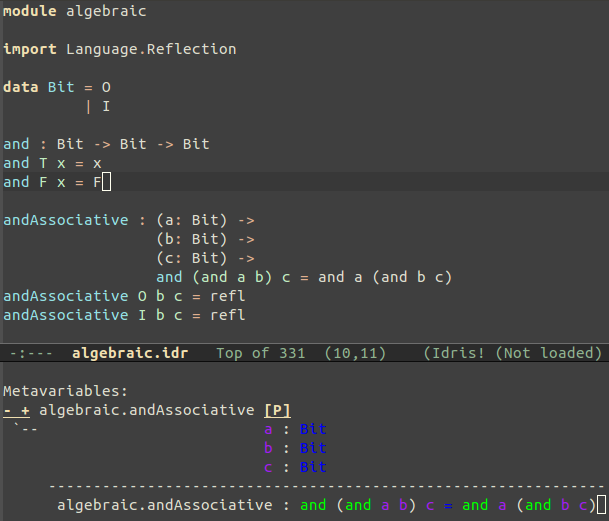
\includegraphics[scale=0.28]{./images/idris.png}
  \end{center}
\end{frame}
